\documentclass[10pt, oneside, letterpaper]{article}
\usepackage[margin=1in]{geometry}
\usepackage[english]{babel}
\usepackage[utf8]{inputenc}
\usepackage{xcolor}
\definecolor{mygreen}{rgb}{0,0.6,0}
\definecolor{mygray}{rgb}{0.5,0.5,0.5}
\definecolor{mymauve}{rgb}{0.58,0,0.82}
\usepackage{listings}
\lstset{
  backgroundcolor=\color{white}, % choose the background color
  basicstyle=\footnotesize\ttfamily, % size of fonts used for the code
  breaklines=true, % automatic line breaking only at whitespace
  frame=single, % add a frame
  captionpos=b, % sets the caption-position to bottom
  commentstyle=\color{mygreen}, % comment style
  escapeinside={\%*}{*)}, % if you want to add LaTeX within your code
  keywordstyle=\color{blue}, % keyword style
  stringstyle=\color{mymauve}, % string literal style
}
\usepackage{enumitem}
\usepackage{blindtext}
\usepackage{datetime2}
\usepackage{fancyhdr}
\usepackage{amsmath}
  \newcommand{\angstrom}{\textup{\AA}} % for units of angstrom
\usepackage{arydshln} % dash line package for matrices
\usepackage{mathtools} % for things like \Aboxed
\usepackage{float}
\usepackage{pgf}
\usepackage{enumitem} % to easily change style of counters in item lists
\usepackage{xurl} % to easily insert URLs in the LaTeX source
\usepackage{braket} % for bra-ket notation
\usepackage{bm} % for bold vector variables
\usepackage{cases} % for piecewise definitions
\usepackage[makeroom]{cancel} % for crossing out terms
\usepackage{graphicx} % for \scalebox
  \newcommand\scalemath[2]{\scalebox{#1}{\mbox{\ensuremath{\displaystyle #2}}}}
\usepackage{textgreek} % enable greek characters in text mode

\setcounter{MaxMatrixCols}{32} % increase the maximum number of matrix columns

\title{Assignment 3}
\author{Calculating Electronic Structures \\ of the Helium atom and Hydrogen Molecule using Basis Functions}
\date{Due: 2022/03/04}

\pagestyle{fancy}
\setlength{\headheight}{23pt}
\setlength{\parskip}{1em}
\fancyhf{}
\chead{Assignment 3}
\rhead{Michel Kakulphimp \\ Student \#63542880}
\lhead{ELEC542 \\ UBC MEng}
\cfoot{\thepage}

\begin{document}
\maketitle
\thispagestyle{fancy}

\section{Directions}

This is a direct follow-up to assignment 2. We are interested in solving the same two systems (hydrogen molecule and helium atom) as in that assignment and comparing the results with what we obtained there.

In this assignment, use the Roothaan equation. As basis functions, use two s-type, normalized Gaussian functions (with different values of \textalpha) centered on each atom. Note that you can choose whatever values of \textalpha you find most suitable for the two Gaussian functions on each atom. Play around with a few different \textalpha values to see which ones give you the most reasonable answers. If you are ambitious, include additional basis functions.

\begin{enumerate}[label=(\alph*)]
  \item (4 points) Describe your approach and show the steps of your derivation all the way to obtaining the matrix equation.
  \item (4 points) Write a computer code to implement what you built in part a.
  \item (4 points) Plot several molecular orbitals and give their associated energies for the helium atom. Also calculate the total energy of the system. Discuss your results.
  \item (4 points) Plot several molecular orbitals and give their associated energies for the hydrogen molecule. Also calculate the total energy of the system (not including the nucleus-nucleus interaction). Discuss your results.
  \item (4 points) Compare your results of both the above exercise and what you obtained in assignment 2 together and also with values available from the literature, and what you obtain using a commercial program such as Gaussian (run through ABACUS, for example).
\end{enumerate}

\section{Derivation of Solution}

As with the previous assignment, since both subjects for this assignment have an even number of electrons that close shells, we can use the restricted Hartree-Fock equation for closed shell systems to numerically calculate the resulting orbitals. The equation is as follows:

\begin{align*}
  \hat{F}(\vec{r})\psi_n(\vec{r}) &= \epsilon_n\psi_n(\vec{r})
\end{align*}

Where $\hat{F}(\vec{r})$ is the Fock operator which is defined as follows:

\begin{align*}
  \hat{F}(\vec{r}) &= \hat{H}_{core}(\vec{r}) + \sum_{n=1}^{N/2}\left[2J_n(\vec{r}) - K_n(\vec{r})\right]\\
\end{align*}

In the previous assignment, the wave equation $\psi_n(\vec{r})$ was obtained by discretizing the solution of the wave equation into a three-dimensional grid partition of size $N \times N \times N$ where each dimension was partitioned into $N$ elements. The Hartree-Fock equation was manipulated to create a matrix eigenvector/eigenvalue problem out of the wave equation to be solved iteratively by a computer program over this space. The largest computational load in the previous assignment's program turned out to be the integration that needed to be performed for every iteration. The exchange term has an integral to calculate over the $N \times N \times N$ space of the matrix. This meant that for every element in the $N \times N \times N$ space, the integration had to be performed over a space of $N \times N \times N$. This integral alone resulted in $N^6$ calculations during every iteration of the Hartree-Fock algorithm. Multiprocessing helped alleviate some of this load by spreading it across multple processing units, but the problem was still very taxing to a modern computer with a modest number of spatial partitions.

This assignment aims to simplify the Hartree-Fock procedure by introducing the concept of basis functions. Known as the Roothaan-Hall equations, the Hartree-Fock equation is augmented by using a combination of non-orthonormal spatial basis functions. The Hartree-Fock procedure is now modified to converge on the coefficients of these basis functions which linearly combine to approximate the electron orbitals. These functions are chosen very carefully to approximate the orbital that the electrons should exist in, which allows a small combination of them to simulate a real system with high accuracy. Likely more accurate and more stable than what was implemented in the previous assignment. Since there are only a few coefficients to solve for in this basis set of functions, the Hartree-Fock procedure is greatly simplified when put into a matrix eigenvector/eigenvalue problem. The basis functions can be described as follows:

\begin{align*}
  \psi_n(\vec{r}) &= \sum_{\mu = 1}^K C_{\mu n}\phi_\mu(\vec{r}) \qquad n = 1, 2, ... , K
\end{align*}

A complete set of functions $\phi_\mu$ could exactly represent a system; however, for computational practicality much less can be used, as is evident by this assignment only asking for two or more. Specifically, normalized gaussian functions are to be used in this assignment. When combined, two or more gaussian functions can better approximate the shape of an atomic orbital as a single gaussian function alone does not match the shape of an atomic orbital very well, which have a pointed asymptotic shape in the middle. By adding a combination of gaussian functions together, the pointed shape is better approximated. An advantage of using a combination of gaussian functions is that they are easily integrated. Since integration is a common operation in Hartree-Fock, this lends well to a rapid calculations towards a convergence.

% Looks like we'll use STO-2G or STO-3G basis sets for this problem.

\newpage
\section{Program Implementation}


\newpage
\section{Results}

\begin{figure}[H]
  \begin{center}
    % 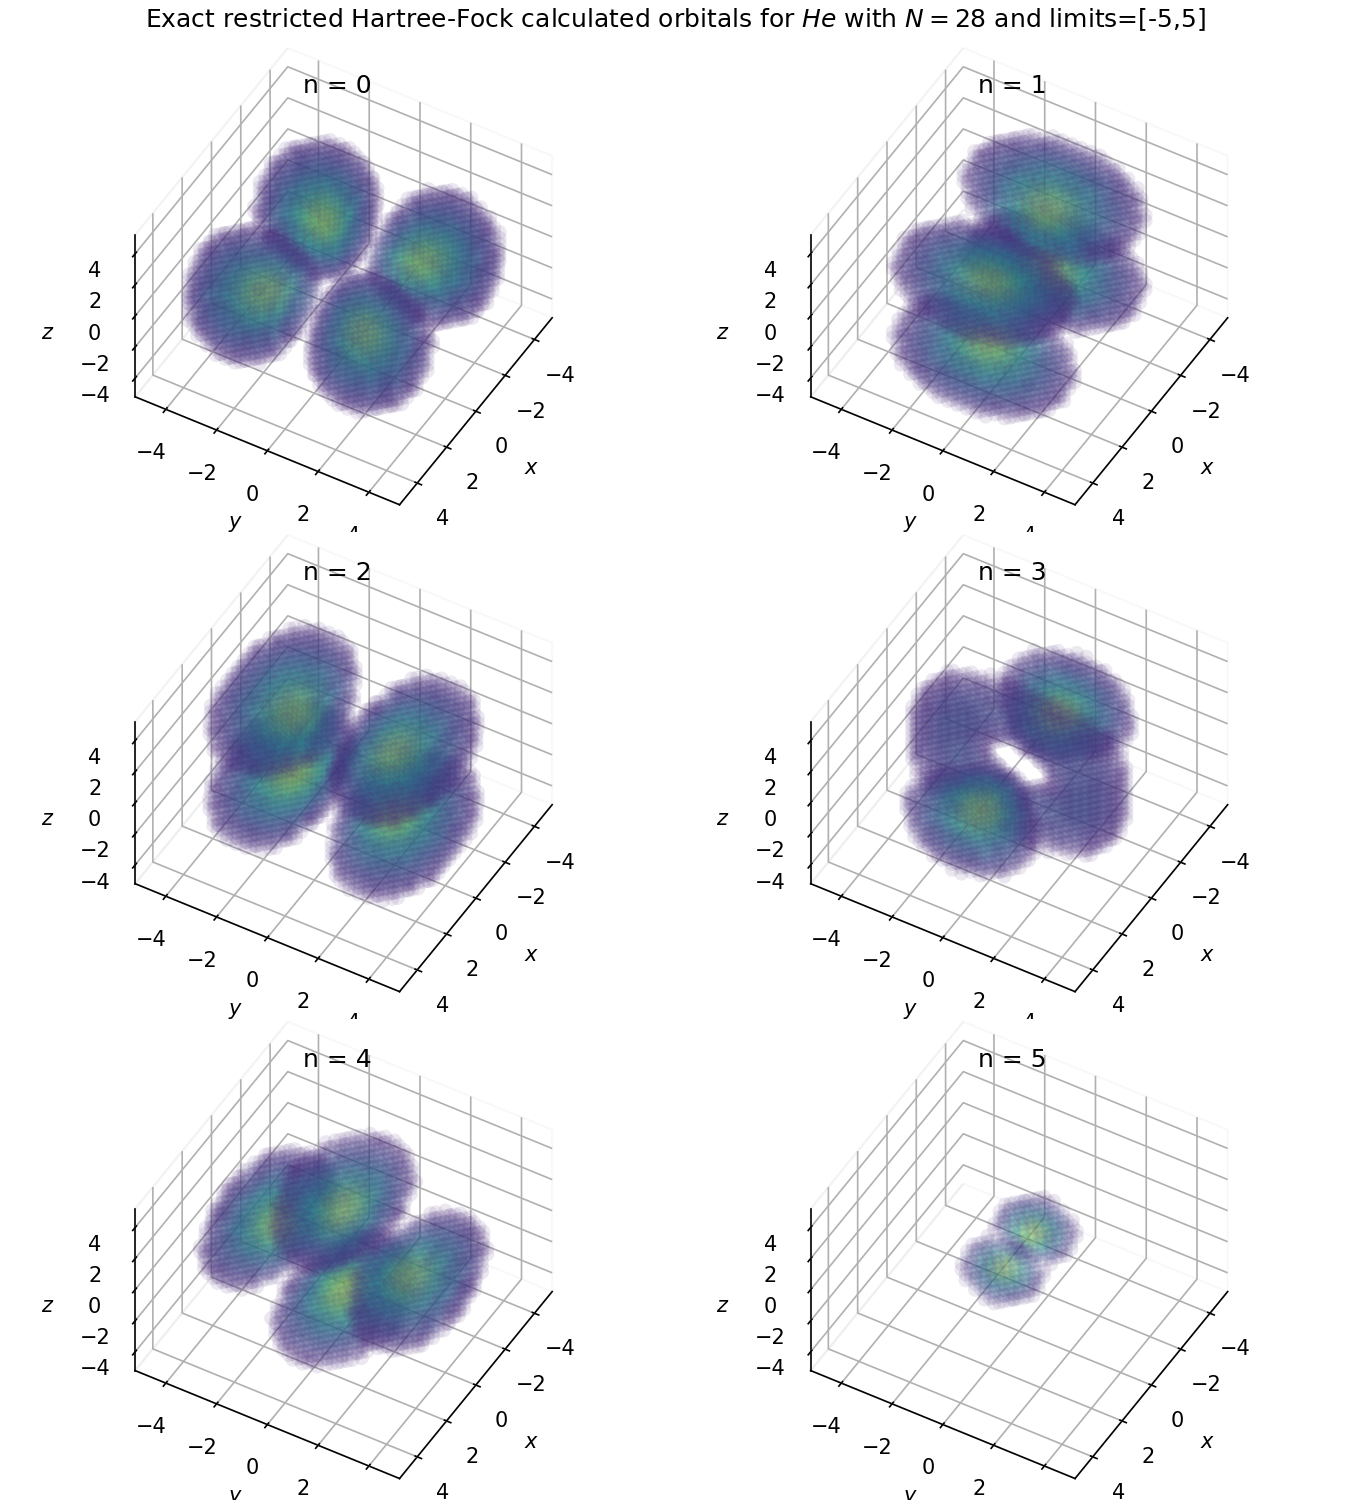
\includegraphics[scale=0.75]{he_N28_l5.png}
  \end{center}
  \caption{Calculated orbitals for $He$ atom using limits of [-5,5]}
  \label{he-plot}
\end{figure}

\begin{table}[H]
\begin{center}
\begin{tabular}{l|llllll}\hline
$n$    & $1$    & $2$     & $3$     & $4$      & $5$      & $6$      \\\hline
$E_n$  & $-0.049968$  & $-0.049878$  & $-0.041970$  & $0.011558$  & $-0.007816$  & $0.065703$ \\\hline
\end{tabular}
\end{center}
  \caption{The first six orbital energy levels obtained from applying HF to the Helium atom using limits of [-5,5]}
  \label{orbital-energies-he}
\end{table}

\newpage
\section{Discussion}

\begin{itemize}
    \item 
\end{itemize}

\newpage
\section{Code Listings and Data}

\subsection{Python Code Listing}
\label{code-listing-python}
The following is the code written in Python to generate the solutions and plots used in this report.
% \lstinputlisting[language=Python]{exact-hartree-fock-sim.py}

\newpage
\section{References}

These aren't citing anything, but they were useful in helping me figure out this assignment.

\begin{itemize}
  \item \url{https://chem.libretexts.org/Courses/Pacific_Union_College/Quantum_Chemistry/11%3A_Computational_Quantum_Chemistry/11.02%3A_Gaussian_Basis_Sets} % Gaussian Basis Sets
  \item \url{https://adambaskerville.github.io/posts/HartreeFockGuide/}
  % Other not relevant
  % \item https://physics.stackexchange.com/questions/20703/why-does-iteratively-solving-the-hartree-fock-equations-result-in-convergence
  % \item https://scicomp.stackexchange.com/questions/1297/why-does-iteratively-solving-the-hartree-fock-equations-result-in-convergence
  % \item https://nznano.blogspot.com/2018/03/simple-quantum-chemistry-hartree-fock.html % basis
  % \item https://github.com/CrawfordGroup/ProgrammingProjects
  % \item https://github.com/aromanro/HartreeFock
  % \item https://github.com/ipudu/SCFpy % solves using a basis set, can't use
  % \item https://medium.com/analytics-vidhya/practical-introduction-to-hartree-fock-448fc64c107b % solves using a basis set, can't use
\end{itemize}

\end{document}

